% !TeX root = main.tex
\chapter{Theoretical Background}

Topics to consider when starting the Sensor Health Monitoring process are mainly that of providing a structured overview of the Sensor Metadata which in itself consists of many layers as a dynamically generated set of metadata is desired. This should be able to accomodate changing Data Acquisitioning (DAQ) System configuration changes.
Consideration is given to the SOIL data model and its' ability to accomodate the many demands that are expected of
sensor data management. \cite{Bodenbenner.2021}
The second major part to consider is that of physical crossrelations and \"deep checks\" which are a experimental mode of checking for inconsistencies among the data.
Major research and implementation work shall go into developing a dynamic model that is generated from the data and then checks back upon the data for possible discrepancies. This approach is chosen as it is estimated to be the most structured approach for a first prototype.



\begin{figure}[h]
         \centering
         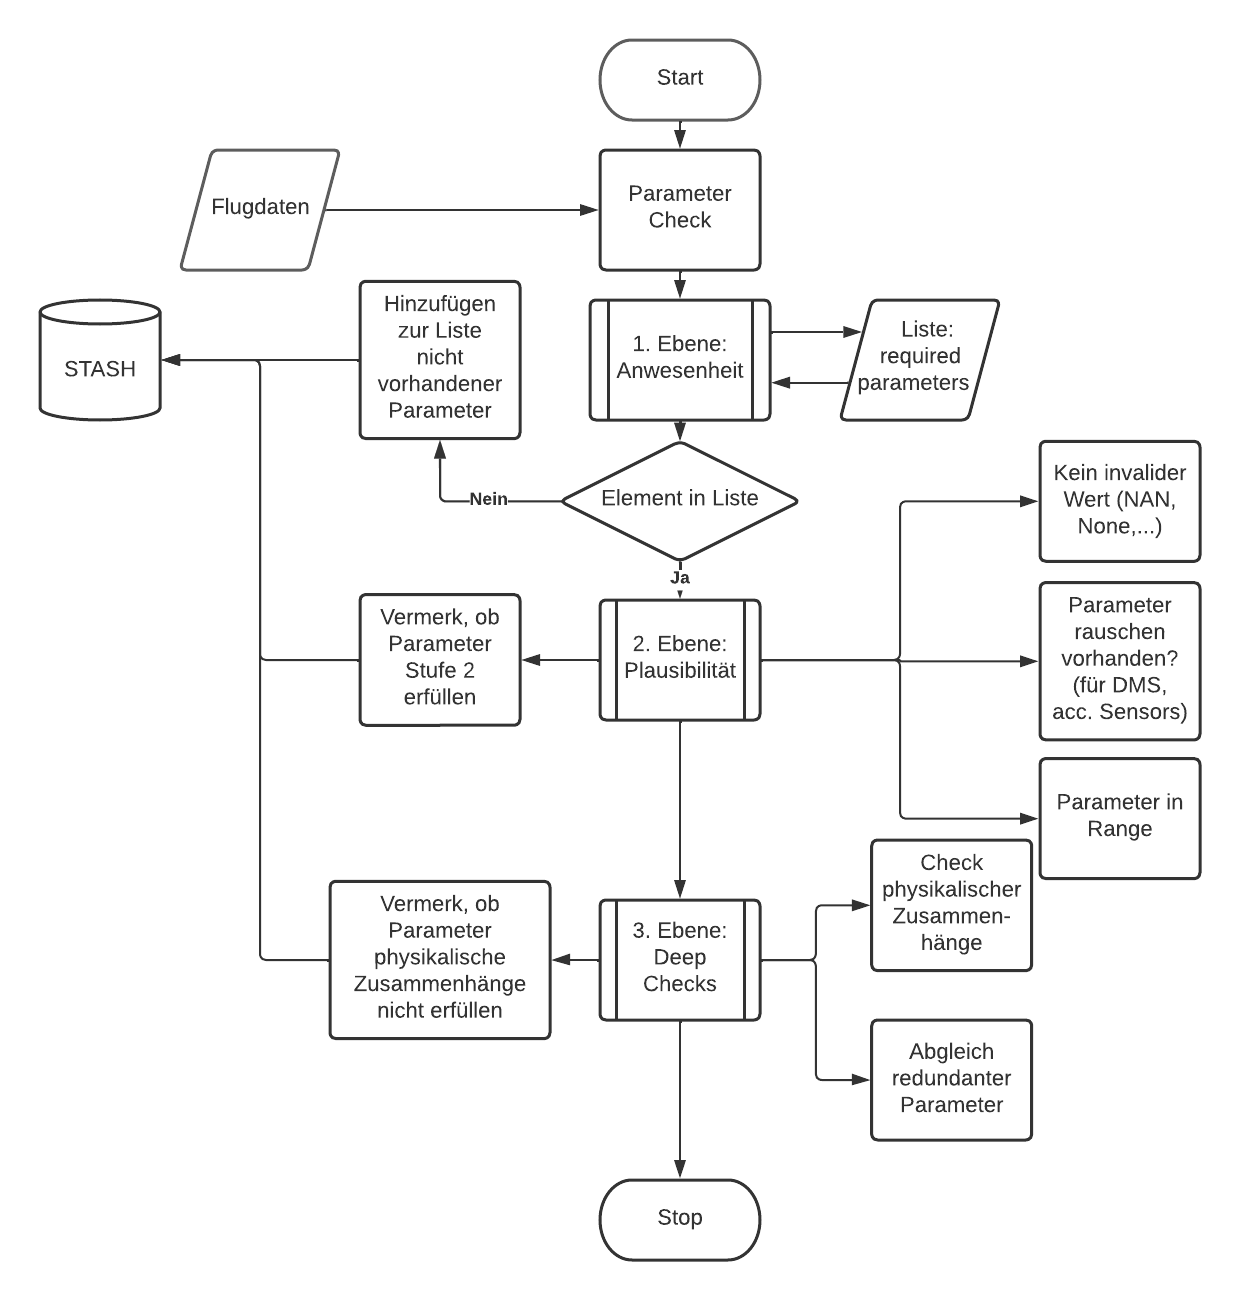
\includegraphics[width=1\textwidth]{SensorHealthMonitoring}
         \caption{}
         \label{fig:}
\end{figure}



\section{Sensor Errors: A quick recap(See Engineers guide to Signal Processing)}
Definition Fault Detection + Fault Diagnosis (Fault-Diagnosis Applications)


Sensors generally produce errors within expected forms of output.
-Noise
    -Measure using Covariance --> autocovariance
-Offset
-No response

Statistical representation of:
Mean

\cite[S.13-17]{Smith.2006}

Time continuous mean
\begin{equation}
    \label{eq:mean_cont}
    \mu=\frac{1}{T} \cdot \int_T x(t) d t
\end{equation}
Time discrete mean:
\begin{equation}
    \label{eq:mean_disc}
\mu=\frac{1}{N} \cdot \sum_{i=1}^{N} x_i
\end{equation}




The variance $\sigma^2$ is a metric for the signal's behaviour. It expresses the mean squared deviation from the mean.

Time
\begin{equation}
    \label{eq:var_cont}
    \sigma^2=\frac{1}{T} \cdot \int_T[x(t)-\mu]^2 d t\\
\end{equation}

\begin{equation}
    \label{eq:var_disc}
\sigma^2=\frac{1}{N} \cdot \sum_{i=0}^{N}\left[x_i-\mu\right]^2
\end{equation}

The standard deviation is derived from the variance. Its value gets square-rooted to better represent the power (magnitude of the amplitude).

Standard Deviation
\begin{equation}
    \label{eq:stdev_disc}
    \sigma = \sqrt{\sigma^2}
\end{equation}

Mean and the standard deviation don't represent the desired metrics in some use cases. Rather more important is a comparison between the two. Hence, the Signal-to-Noise ratio (SNR) is used to compare and condense the mean and standard deviation by dividing the mean by the standard deviation.

\begin{equation}
    \label{eq:snr}
    SNR=\frac{\mu}{\sigma^2}
\end{equation}
 Another parameter is the coefficient of variation (CV) which is the standard deviation divided by the mean and multiplied by 100\%.

\begin{equation}
    \label{eq:coeff_var}
    CV = \frac{\sigma^2}{\mu}100\%
\end{equation}

An arising problem based on the SNR and CV are however that they scale based on the mean value. Should the mean value lie at about 0 for e.g. a sensor of an aircraft control surface, the signal to noise ratio will be relatively high compared to an acceleration sensor in z axis with a constant offset of 1g

Practical example for noise, sinus wave, superposed sinus wave
\begin{figure}[h]
         \centering
         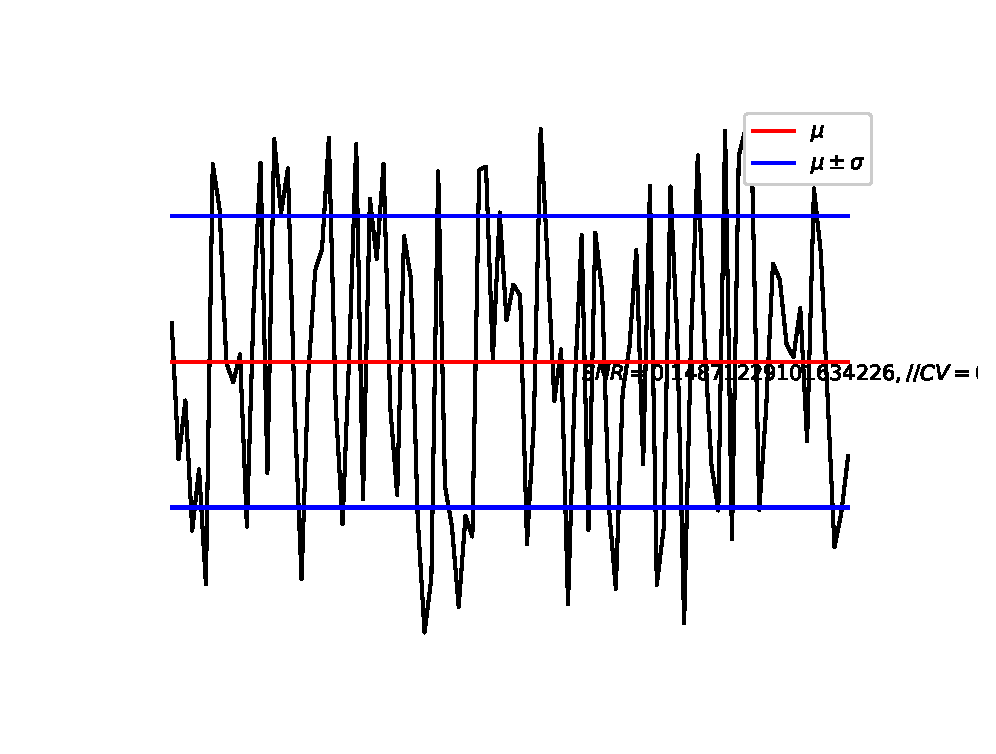
\includegraphics[width=.7\textwidth]{python_functions/images/basic_signal_0}
         \caption{Mean and standard deviation for a white noise signal}
         \label{fig:signal_basic}
\end{figure}

To evaluate a signal according to the quantitiesThe next logical step for statistic Histogram

probability mass function



Covariance
-->Autocovariance

Correlation


stft.

Test noise analysis over short time window of 256 samples.

Define here





Also, next to the simple and known models to display an error is the Luenberger Beobachter.
enter placeholder for image: Measurement equals signal + error
and image: luenberger beobachter. Kalman Implementierung (Lie13)
Parameter Correlation Studies (Li15)

\section{Integrity, Reliability and Validity based on GNSS}
Data according to ISO 8000 cite [ISO22]
iso5725:
-accuracy(validity)+precision(reliability)
Also see precision and accuracy definition \cite[S.33ff.]{Smith.2006}


cite faa08
B.1.5: Reliability = 1-Probability_Failure

B.1.10: Integrity: Display when system should not be used due to potential errors.

Validation: Black Box Testing. Results match expectations
Verification: White Box Testing. Establish algorithm's truth




\section{control systems approach}

Following the recipe for a modeled aircraft based on sensor data we try to simulate the parameters x and u of the aircraft with the sensor data y. Khaled shows that this approach works for linking omega_x omega_y, delta_delta(drift angle) with omega_z. and Transmissibility function  $\mathcal{T}$


The examined approaches include:
\begin{enumerate}
    \item Transmissibility functions $\mathcal{T}$ that model the system output without having to take the unknown
    system input into consideration
    \item Bond Graphs to model a physical rigid aircraft system
    \item Physical relations
    \item redundancies between sensors
\end{enumerate}

\section{Intro existing architectures}

\section{Data Format, FAIR}
json file format (FAIR-principles, INST-DLR, SOIL)

Explain which means are taken to guarantee an architecture throughout the work that ensures an implementation of the FAIR principles and the V-model.
Architecture of the JSON-Tree structure and which data is inserted where.


-modern data management principles (storage not as important as readability)

Comparison with existing data structures. Implementation into existing architecture

--> Chosen Data Model, Semantics

\section{Faults}

Fault definition from [Isermann(20)][HALO-Report]

\section{Stash}

\section{downloadfunctionalities}
file sizes too large --> Reduction for on demand parameters and resampling utility
Handling of large data sets


\section{Software architecture considerations}

Careful consideration needs to be given to the workflow of the level 1 check to allow scalability and minimal manual interaction in later stages. To achieve this architecture, manual steps are reduced as far as possible.


\section{DAQs, ISTAR}
    DLR data generation (DAQs) (How Data is checked)

Matthews flowchart(dataflow from sensor voltage through computer-computer-user)
Exemplary for a single sensor



\section{Level 1 Implementation}

For implementing the level 1 checks, the measured data needs to be compared to the expected data. To gain insight into what the the expected data is, the configuration file of the data acquisitioning system needs to get parsed.
Luckily, the DAQ's format is a .zip directory.
The 7zip command line tool gets used for opening the configuration file since the configuration file's format is not fully complying to the zip standard making several python libraries fail during the process. This stems from an issue with the zip header and footer parts of the file that are not at expected places (i.e.\ the front the back).
Once opened, the configuration file contains multiple files as well as an essential xml file that contains the needed sensor metadata.

Missing datasets can now easily be found by comparing the expected values from the configuration file to the actual generated data.

For the second step.

\section{Level 2 Implementation}

Since the IMC DAQ System resamples the 20Hz Sensors to a straight timeframe data gets lost in the process. This makes potentially noisy sensors output the same value twice in a row since the DAQ hasn't yet received the new sensor data and outputs the same value multiple times in a row. Even sensors with a high noise ratio such as the fine part of a gps latitude signal outputs the same value twice in a row which is highly unlikely to happen on a statistical basis. Since this occurs quite often the question arises if the actual sampling may be lower than the actual data.


\section{Level 3 Implementation}

Aims of Level 3 Implementation are to model the aircraft's state in a reference system.
This reference system shall be geodetic and fixed to the earth while the aircraft moves through it. Moving aircraft coordinate systems like the aerodynamic and the along track Coordinate system may be derived from its geodetic position using ?angles and velocities.


\section{Deep dive into altitudes}

The aircraft altitude generally is defined as the displacement of the aircraft from sea level.
On a geodetic scale, the earth can be described as an ellipsoid due to its rotation. However, varying density levels of the earth's crust cause the elevation and sea level to deviate from the ellipsoid shape. This results in a lopsided model that is modeled in the WGS84 (ref and image here) system. This is also the altitude that the gps measures. And will be the reference altitude for the following calculations.

The main existing altitudes are the:
\begin{enumerate}
    \item Geodetic Altitude (GNSS)
    \item Barometric Altitude (used in conjunction with reference pressure)
    \item Inertial Altitude
    \item Radar Altitude (can be used in conjunction with a terrain model to derive geodetic altitude)
\end{enumerate}
Possible errors for each are:
geodetic: inconvenient satellite placements, deflection of signals in the atmosphere and signal problems
Barometric Altitude: Possible errors due to drift and meteorological atmospherical pressure shifts, Reference Altitude.

Going into WGS84 and the GNSS Altitude however exceeds the scope of this work. In the following, the satellite altitude above Mean Sea Level (MSL) is considered as the reference altitude.


